\documentclass[12pt,a4paper]{report}
\usepackage[utf8]{inputenc}
\usepackage[english,russian]{babel}
\usepackage{indentfirst}
\usepackage{pdfpages}
\usepackage{titlesec}
\usepackage{listings}
\usepackage{amsmath}

% Вставка картинки
\usepackage{graphicx}
\graphicspath{{schemes/}}
\DeclareGraphicsExtensions{.pdf,.png,.jpg}

\usepackage[tableposition=top,singlelinecheck=false]{caption}

\usepackage[14pt]{extsizes}

\newcommand{\hsp}{\hspace{20pt}}
\titleformat{\chapter}[hang]{\large\bfseries}{\thechapter{. }}{0pt}{\large\bfseries}
\titlelabel{hlabel-formati}
\titlespacing{\chapter}{42pt}{-20pt}{12pt}
\titleformat{\section}[hang]{\large\bfseries}{\thesection{. }}{0pt}{\large\bfseries}
\titlespacing{\section}{42pt}{12pt}{5pt plus 5pt}

% Отступ абзаца
\usepackage{indentfirst}
\setlength{\parindent}{1.5cm}

% Межстрочный интервал
\usepackage{setspace}
\onehalfspacing % интервал 1.5

\usepackage[left=3cm, right=1cm, top=2cm, bottom=2cm]{geometry}

\AtBeginDocument{%
	\renewcommand\contentsname{Содержание}
}

\begin{document}
% Титульник
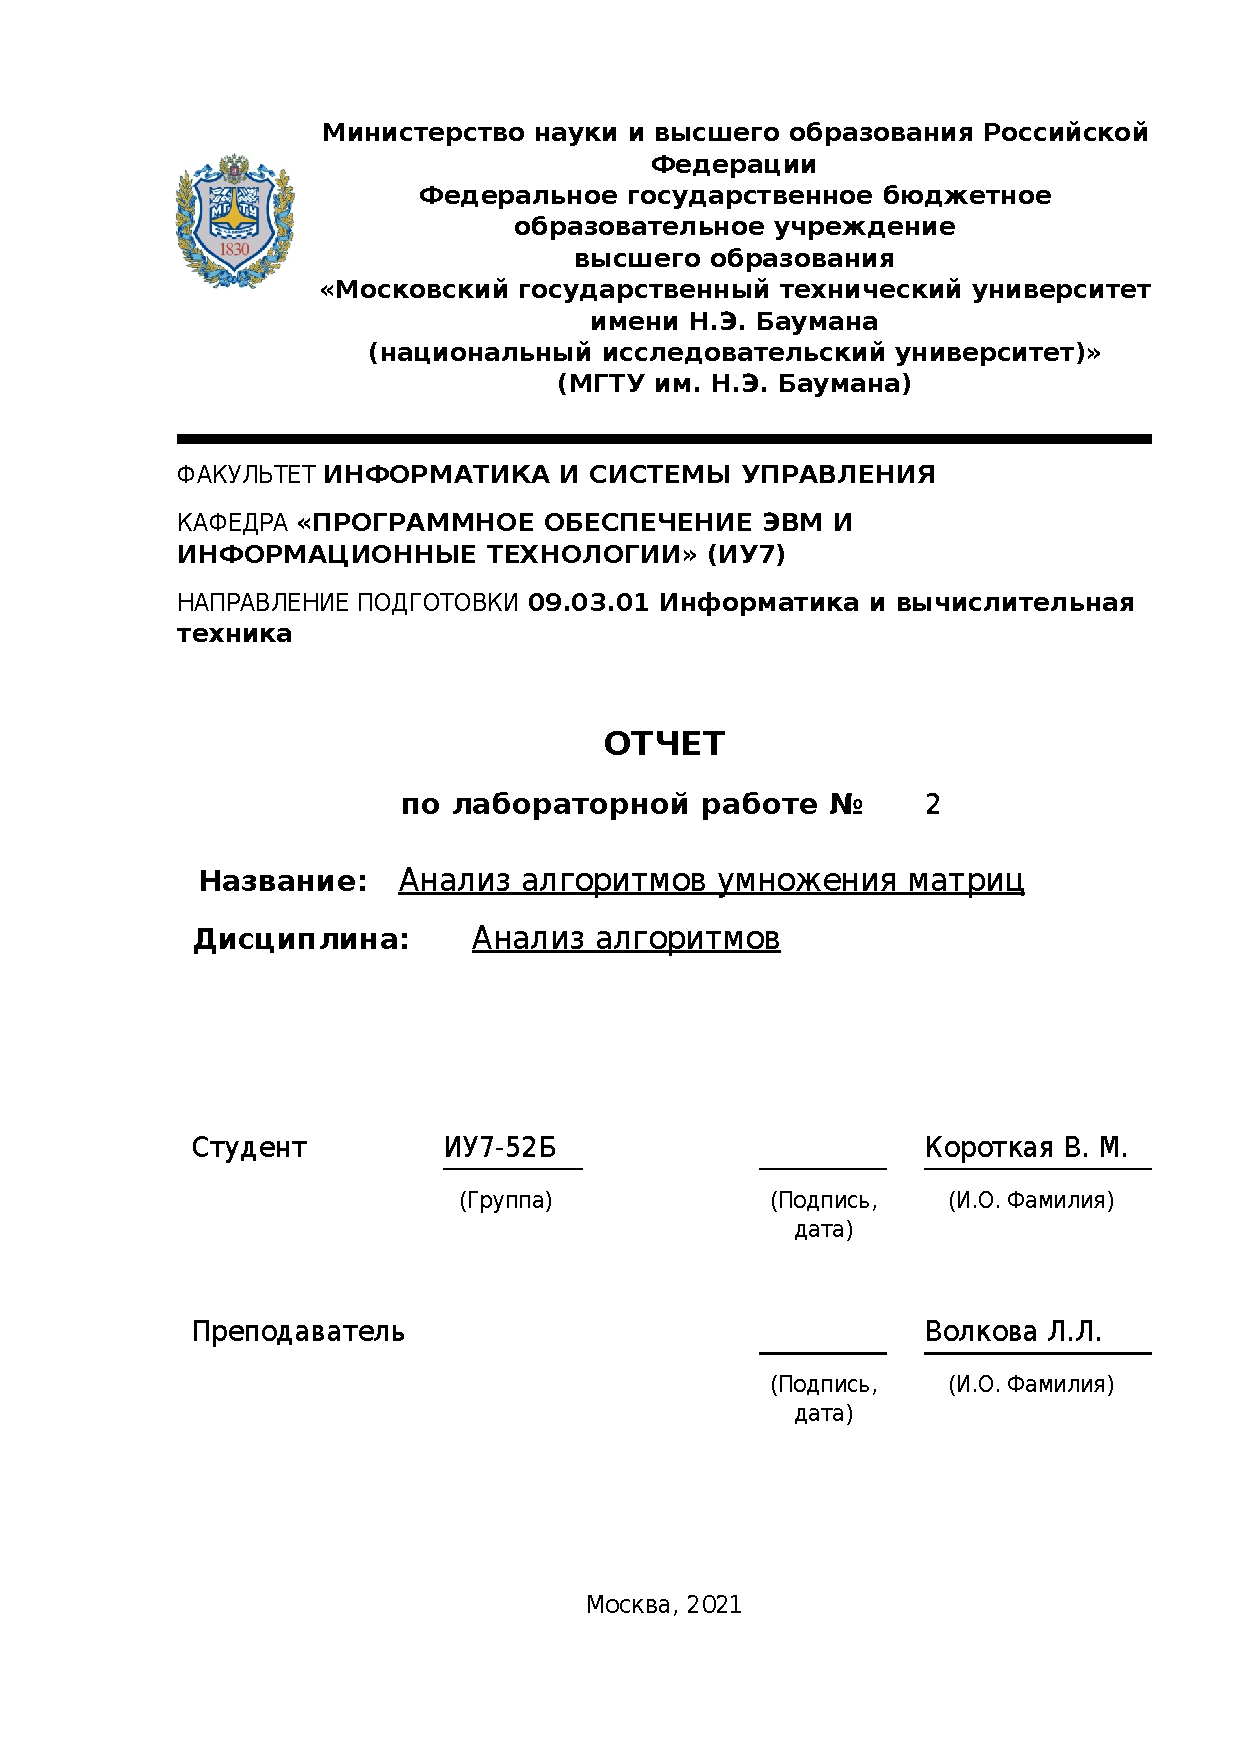
\includepdf[pages=1]{titul.pdf}
% Оглавление
\tableofcontents

\newpage
\chapter*{Введение}
\addcontentsline{toc}{chapter}{Введение}
В этой лабороторной работе мы рассматриваем вопрос, который часто
\textbf{Умножение матриц} - это один из базовых алгоритмов, который широко применяется в различных численных 
методах, и в частности в алгоритмах машинного обучения. 
Многие реализации прямого и обратного распространения сигнала в сверточных слоях неронной сети базируются на 
этой операции. Для перемножения двух матриц необходимо, чтобы количество столбцов в первой матрице совпадало 
с количеством строк во второй. У результирующей матрицы будет столько же строк, сколько в первой матрице, и 
столько же столбцов, сколько во второй. 

Сложность вычисления произведения матриц по определению составляет $O(n^3)$, однако существуют более эффективные 
алгоритмы, которые применяются для больших матриц. 
Вопрос о предельной скорости умножения больших матриц, также как и вопрос о построении наиболее быстрых и усточивых 
практических алгоритмов умножения больших матриц остаётся одной из нерешённых проблем линейной алгебры.

Цель данной лабораторной работы заключается в изучении алгоритмов умножения матриц.
Рассматриваются стандартный алгоритм умножения матриц, а также алгоритм Винограда и модифицированный алгоритм 
Винограда.
Требуется рассчитать и изучить затрачиваемое каждым алгоритмом время. 

В данной лабораторной работе выделено несколько задач:
\begin{itemize}
	\item изучить алгоритмы умножения матриц: стандартный и алгоритм Винограда;
	\item модифицировать алгоритм Винограда;
	\item дать теоретическую оценку базового алгоритма умножения матриц, алгоритму Винограда и модифированному алгоритму Винограда;
	\item реализовать три алгоритма умножения матриц на одном из языков программирования;
	\item сравнить алгоритмы умножения матриц.
\end{itemize}

\newpage
\chapter{Аналитическая часть}

В данном разделе будут рассмортенно формальное описание алгоритмов.

\section{Стандартный алгоритм умножения матриц}

Пусть даны две матрицы A и B с размерностями $m\times n$ и $n\times l$ соответственно (1.1) и (1.2):

\begin{equation}
    \begin{bmatrix} 
        a_{1,1}      & \textrm{...} & a_{1,n} \\
        \textrm{...} & \textrm{...} & \textrm{...} \\
        a_{m,1}      & \textrm{...} & a_{m,n}
    \end{bmatrix}
\end{equation}

\begin{equation}
    \begin{bmatrix} 
        b_{1,1}      & \textrm{...} & b_{1,l} \\
        \textrm{...} & \textrm{...} & \textrm{...} \\
        b_{n,1}      & \textrm{...} & b_{n,l}
    \end{bmatrix}
\end{equation}


В результате умножения, получим матрицу C размерностью $m\times l$ (1.3):

\begin{equation}
    \begin{bmatrix} 
        c_{1,1}      & \textrm{...} & c_{1,l} \\
        \textrm{...} & \textrm{...} & \textrm{...} \\
        c_{m,1}      & \textrm{...} & c_{m,l}
    \end{bmatrix}
\end{equation}

$c_{i,j}=\sum\limits_{r=1}^n a_{i,r} \cdot b_{r,j}$ называется произведением матриц A и B.

\section{Алгоритм Винограда}

Если посмотреть на результат умножения двух матриц, то видно, что каждый элемент в нем представляет 
собой скалярное произведение соответствующих строки и столбца исходных матриц. 
Можно заметить также, что такое умножение допускает предварительную обработку, позволяющую часть работы 
выполнить заранее. \\

Рассмотрим два вектора $V = (v_{1}, v_{2}, v_{3}, v_{4})$ и $W = (w_{1}, w_{2}, w_{3}, w_{4})$. Их 
скалярное произведение (1.4). 
\begin{equation}
    V \cdot W = v_{1} \cdot w_{1} + v_{2} \cdot w_{2} + v_{3} \cdot w_{3} + v_{4} \cdot w_{4}
    \label{formula:1}
\end{equation}

Это равенство можно переписать в виде ()\ref{formula:2})
\begin{equation}
    V \cdot W = (v_{1} + w_{2})(v_{2} + w_{1}) + (v_{3} + w_{4})(v_{4} + w_{3}) - v_{1} \cdot v_{2} - v_{3} \cdot v_{4} - w_{1} \cdot w_{2} - w_{3} \cdot w_{4}
    \label{formula:2}    
\end{equation}

Кажется, что формула \ref{formula:2} задает больше работы, чем первое: вместо четырех умножений мы насчитываем их 
шесть, а вместо трех сложений - десять.
Менее очевидно, что выражение в правой части последнего равенства допускает предварительную обработку: его 
части можно вычислить заранее и запомнить для каждой строки первой матрицы и для каждого столбца второй. 
На практике это означает, что над предварительно обработанными элементами нам придется выполнять лишь первые 
два умножения и последующие пять сложений, а также дополнительно два сложения.

\section*{Вывод}

В данном раздели были рассмотрены алгоритмы умножения матриц.
Алгоритм Винограда предлагает подсчитывать значения заранее перед основными вычислениями, что может повысить 
производительность при перемножении достаточно больших матриц. 
Однако с малыми размерами, он может справляться хуже чем другие, но алгоритм можно оптимизировать и добиться 
более высокой скорости подсчёта.


Входными данными реализуемого ПО являются:

\begin{itemize}
	\item размерность первой матрицы - два натуральных числа;
	\item первая матрица - целочисленная;
	\item размерность второй матрицы - два натуральных числа;
	\item вторая матрица - целочисленная.
\end{itemize}

Выходными данными реализуемого ПО являеться результат алгоритмов умножения матриц т. е.:
\begin{itemize}
	\item матрица (результат) - для классического умножения матриц;
	\item матрица (результат) - для алгоритма Винограда;
	
\end{itemize}
Ограничением для реализуемого ПО является - размерность вводимых матриц т. е. длинна строки первой матрицы должна совпадать с длинной колонки второй матрицы.

\newpage
\chapter{Конструкторская часть}

В данном разделе представлены схемы алгоритмов. Так же будут описаны пользовательские структуры данных, приведены структура ПО и классы эквивалентности для тестирования реализуемого ПО.



\section{Схемы алгоритмов}

На рисунке 2.1 представлена схема классического алгоритма умножения матриц.

\begin{figure}[ht]
	\center{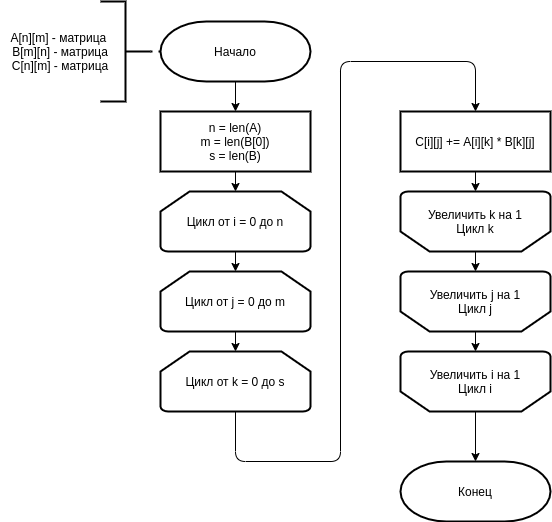
\includegraphics[scale=0.8]{classic}}
	\caption{Классический алгоритм умножения матриц.}
	%\label{fig:image}
\end{figure}'

На рисунках 2.2-2.3 представлена схема алгоритма Винограда умножения матриц.

\begin{figure}[ht!]
	\center{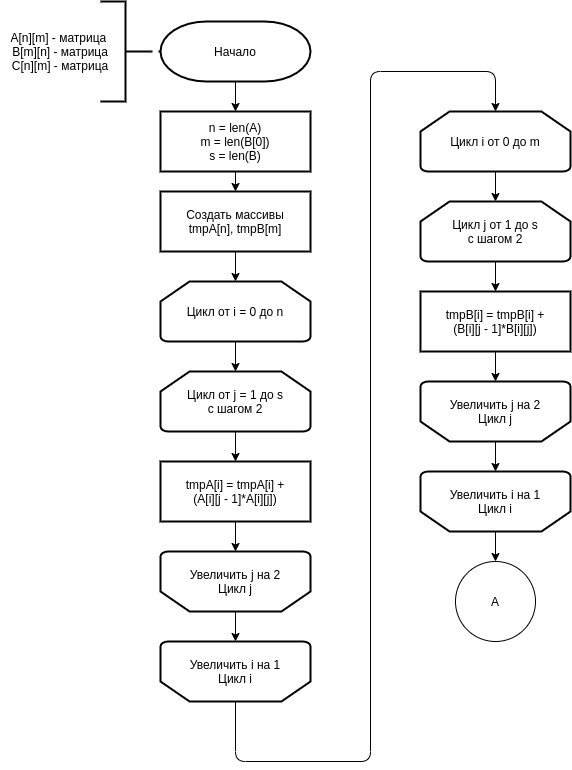
\includegraphics[scale=0.8]{vinograd1}}
	\caption{Алгоритм Винограда умножения матриц(часть 1)}
	%\label{fig:image}
\end{figure}

\begin{figure}[ht!]
	\center{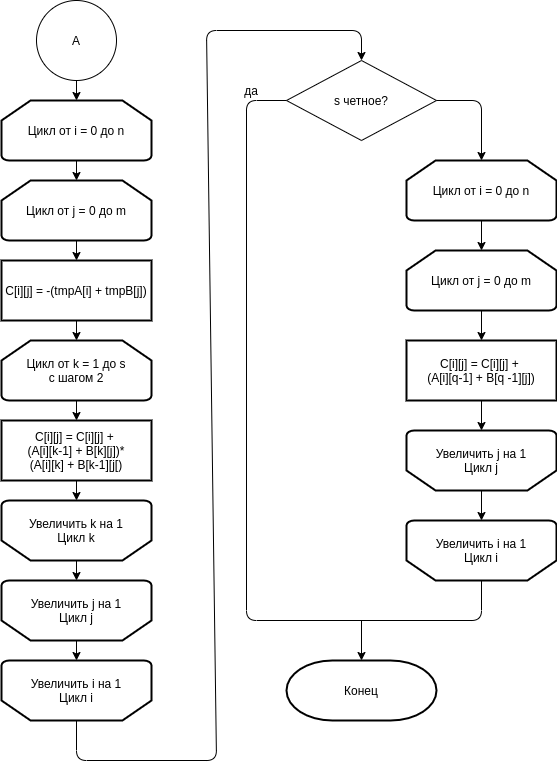
\includegraphics[scale=0.8]{vinograd2}}
	\caption{Алгоритм Винограда умножения матриц(часть 2)}
	%\label{fig:image}
\end{figure}

\section{Структура ПО}

На рисунке 2.5 представлена диограмма классов.

\section*{}
\begin{figure}[ht]
	\center{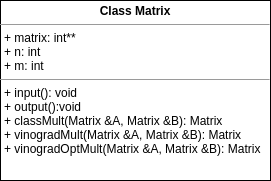
\includegraphics[scale=0.8]{structPO}}
	\caption{Диаграмма классов реализуемого ПО}
	%\label{fig:image}
\end{figure}

\section{Тестирование}

В рамках данной лабораторной работы были выделены следующие классы эквивалентности:
\begin{itemize}
	\item входными данными являются две матрицы размерностью 1*1;
	\item входными данными являются две матрицы размерностью 1*n и n*1 соответственно;
	\item входными данными являются две матрицы квадратные матрицы равной размерностью;
	\item входными данными являются две матрицы размерностью n*k и к*т.
\end{itemize}

Для проверки работы программы будет осуществлено тестирование согласно классам эквивалентности.

\section*{Вывод}
       
Были составлены схемы и подсчитана трудоёмкость для каждого алгоритма.
Из последнего можно увидеть, что оптимизированный алгоритм Винограда менее трудоёмкий, чем неоптимизированный.     


\newpage
\chapter{Технологическая часть} 

В данном разделе приведены средства реализации, требования к ПО и листинги кода.

\section{Средства реализации}
В качестве языка программирования был выбран с++. Данный язык знаком и предостовляет все необходимые ресурсы.
В качестве среды разработки я использовала Visual Studio Code, т.к. считаю его достаточно удобным и легким.
Visual Studio Code подходит не только для  Windows, но и для Linux, это еще одна причина, по которой я выбрала VS code, т.к. у меня установлена ОС  fedora 34.

\section{Сведенья о модулях программы}

\begin{itemize}
	\item main.cpp - файл, содержащий точку входа в программу;
	\item matrix.cpp - файл, содержащий реализацию алгоритмов умножения матриц.
\end{itemize}

\section{Реализация алгоритмов}

В листингах 3.1 - 3.3 приведены реализации алгоритмов
сортировки массивов на ЯП C++.

\noindent\textrm{Листинг 3.1: Классический алгоритм умножения матриц.}
\begin{lstlisting}[frame=single, numbers=left]
void Matrix::classicMultiplication(Matrix &A, Matrix &B)
{
  for (int i = 0; i < this->n; i++)
  for (int j = 0; j < this->m; j++)
  for (int k = 0; k < A.column(); k++)
    this->matrix[i][j] += A.matrix[i][k] * B.matrix[k][j];
}
\end{lstlisting}

\noindent\textrm{Листинг 3.2: Алгоритм Винограда.}
\begin{lstlisting}[frame=single, numbers=left]
void Matrix::vinogradMultiplication(Matrix &A, Matrix &B)
{
    precomputeRows(A);
    precomputeCols(B);
	
    for(int i = 0; i < A.row(); i++)
    for (int j = 0; j < B.column(); j++)
    {
        this->matrix[i][j] = -1*(tmpA[i], tmpB[j]);
        for (int k = 0; k < B.row()/2; k++)
        {
            this->matrix[i][j] = this->matrix[i][j] +
            (A.get(i, k*2) + B.get(k*2 + 1, j)) *
            (A.get(i, k*2 + 1) + B.get(k*2 , j));
        }
    }
	
    if (B.row()%2)
    {
        for (int i = 0 ; i < A.row(); i++)
            for (int j = 0; j < B.column(); j++)
            {
                this->matrix[i][j] = this->matrix[i][j] +
                A.get(i, B.row()/2 - 1)*
                B.get(B.row()/2 - 1, j);
        }
    }
	
    delete []tmpA;
    delete []tmpB;
	
}

void Matrix::precomputeRows(Matrix &A)
{
    tmpA = new int [A.row()];
	
    for (int i = 0; i < A.row(); i++)
        for (int j = 0; j < A.column()/2 ;j++)
        {
            tmpA[i] = tmpA[i] + 
            A.get(i, j*2) * A.get(i, j*2 + 1);
        }
}

void Matrix::precomputeCols(Matrix &B)
{
    tmpB = new int [B.column()];
	
    for (int i = 0; i < B.column(); i++)
        for (int j = 0; j < B.row()/2 ;j++)
        {
             tmpB[i] = tmpB[i] +
              B.get(j*2, i) * B.get(j*2 + 1, i);
        }
}
\end{lstlisting}

\noindent\textrm{Листинг 3.3: Оптимизированный алгоритм Винограда}
\begin{lstlisting}[frame=single, numbers=left]
void Matrix::vinogradOptMultipl(Matrix &A, Matrix &B)
{
    precomputeRowsOpt(A);
    precomputeColsOpt(B);
	
    int temp = 0;
	
    for(int i = 0; i < A.row(); i++)
    for (int j = 0; j < B.column(); j++)
    {
        temp = -1*(tmpA[i], tmpB[j]);
        for (int k = 0; k < B.row()/2; k++)
        {
            temp += (A.get(i, k-1) + B.get(k, j)) *
            (A.get(i, k) + B.get(k-1, j));
        }
        this->matrix[i][j] = temp;
    }
	
    if (B.row()%2)
    {
        for (int i = 0 ; i < A.row(); i++)
        for (int j = 0; j < B.column(); j++)
        {
            this->matrix[i][j] += 
            A.get(i, B.row() - 1) * B.get(B.row() - 1, j);
        }
		
    }
	
    delete []tmpA;
    delete []tmpB;
}


void Matrix::precomputeRowsOpt(Matrix &A)
{
    tmpA = new int [A.row()];
	
    for (int i = 0; i < A.row(); i++)
    {
        for (int j = 0; j < A.column() ;j+=2)
        {
            tmpA[i] = A.get(i, j-1) * A.get(i, j);
        }
    }
}

void Matrix::precomputeColsOpt(Matrix &B)
{
    tmpB = new int [B.column()];
	
    for (int i = 0; i < B.column(); i++)
    {
        for (int j = 0; j < B.row() ;j++)
        {
            tmpB[i] = B.get(j-1, i) * B.get(j, i);
        }
    }
}
\end{lstlisting}

\section{Оценка трудоемкости}

Для начала оценки алгоритмов, можно ввести специальную модель трудоёмкости:
\begin{itemize}
	\item стоимость базовых операций 1 — +, -, *, /, =, == \dots ;
	\item оценка цикла — $f_{for} = f_{init} + N \cdot (f + f_{body} + f_{post}) + f$, где 
	f - условие цикла, $f_{init}$ - предусловие цикла, $f_{post}$ - постусловие цикла;
	\item стоимость условного перехода примем за 0, стоимость вычисления условия остаётся.
\end{itemize}

\textbf{Для стандартного алгоритма умножения} с матрицами A и B и размерами $n\times m$ и $m\times l$ 
соответственно: \\

$f = 2 + n \cdot (2 + 2 + l \cdot (2 + 2 + m \cdot (2 + 6 + 2))) = 10nlm + 4ln  + 4n + 2$ \\

\textbf{Для алгоритма Винограда} при тех же матрицах и их размерах. \\

Для более понятного подсчёта, можно составить таблицу (таблица 2.1), а затем подсчитать общую трудоёмкость:

\begin{displaymath}
	f = 13mnl + 7.5mn + 7.5lm + 11ln + 8n + 4l + 14 + \left \{ 
	\begin{array}{ll}  
		0, \textrm{если m чётное} \\ 
		15 \cdot l \cdot n + 4 \cdot n + 2, \textrm{иначе} 
	\end{array} \right.
\end{displaymath}

\begin{table}[h]
	\caption{трудоёмкость алгоритма Винограда}  
	\label{tabular:timesandtenses}
	\begin{center}
		\begin{tabular}{ | l | l | }
			\hline
			Часть алгоритма            & Трудоёмкость                                                        \\ \hline
			Инициализация mulH и mulV  & $2 \cdot 3$                                                         \\ \hline
			Заполнение mulH            & $2 + n \cdot (2 + 2 + m / 2 \cdot (3 + 6 + 6))$                     \\ \hline
			Заполнение mulV            & $2 + l \cdot (2 + 2 + m / 2 \cdot (3 + 6 + 6))$                     \\ \hline
			Подсчёт результата         & $2 + n \cdot (2 + 2 + l \cdot (2 + 7 + 2 + m / 2 \cdot (3 + 23)))$  \\ \hline
			Условный оператор нечёт. m & $2$                                                                 \\ \hline
			Для матриц с нечёт m       & $2 + n \cdot (2 + 2 + l \cdot (2 + 8 + 5))$                         \\ \hline
		\end{tabular}
	\end{center}
\end{table}

\textbf{Для оптимизированного алгоритма Винограда} при тех же матрицах и размерах. 
Для более понятного подсчёта, можно тоже составить таблицу (таблица 2.2).

\begin{displaymath}
	f = 8mnl + 5mn + 5lm + 12ln + 8n + 4l + 18 + \left \{ 
	\begin{array}{ll}  
		0, \textrm{если m чётное} \\ 
		10 \cdot l \cdot n + 4 \cdot n + 4, \textrm{иначе} 
	\end{array} \right.
\end{displaymath}

\begin{table}[h]
	\caption{трудоёмкость оптимизированного алгоритма Винограда}  
	\label{tabular:timesandtenses}
	\begin{center}
		\begin{tabular}{ | l | l | }
			\hline
			Часть алгоритма               & Трудоёмкость                                                            \\ \hline
			Инициализация mulH и mulV     & $2 \cdot 3$                                                             \\ \hline
			Инициализация m1Mod2          & $2 \cdot 2$                                                             \\
			и n2Mod2                      &                                                                         \\ \hline
			Заполнение mulH               & $2 + n \cdot (2 + 2 + m / 2 \cdot (2 + 5 + 3))$                         \\ \hline
			Заполнение mulV               & $2 + l \cdot (2 + 2 + m / 2 \cdot (2 + 5 + 3))$                         \\ \hline
			Подсчёт результата            & $2 + n \cdot (2 + 2 + l \cdot (2 + 5 + 3 + 2 + $                        \\
			& $ + m / 2 \cdot (2 + 14)))$                                             \\ \hline
			Условный оператор нечёт. m    & $2$                                                                     \\ \hline
			Для матриц с нечёт m          & $2 + 2 + n \cdot (2 + 2 + l \cdot (2 + 6 + 2))$                         \\ \hline
		\end{tabular}
	\end{center}
\end{table}

\section{Тестирование}

В данном разделе будет приведена таблица с тестами (таблица \ref{table:ref1}).
% \ref{table:ref1}, в которой четко отражено тестирование программы

\begin{table}[ht]
	\centering
	\caption{Таблица тестов}
	\label{table:ref1}
	\begin{tabular}{ | l | l | l |}
		\hline
		Матрица A       & Матрица B           & Результат                               \\ \hline
		2 2 1 0 0 1     & 2 2 1 0 0 1         & Ответ верный                            \\ \hline
		3 2 2 3 1 0 2 2 & 2 4 2 2 1 9 4 2 8 1 & Ответ верный                            \\ \hline
		2 1 2 1         & 12 12               & Ответ верный                            \\ \hline
		2 2 1 0 0 1     & 1 1 0               & Сообщение о неверном вводе размерностей \\ \hline
		0 0             & 0 0                 &                                         \\ \hline
		\hline
	\end{tabular}
\end{table}

Все тесты пройдены.



\section*{Вывод}

В данном разделе были приведены средства реализации, требования к ПО и листинги кода.

\newpage
\chapter{Исследовательская часть} 

В данном разделе сравним работу каждого алгоритма.

\section{Временные характеристики}

Для сравнения возьмем квадратные матрицы размерностью [10, 20, 30,\dots,100]. 
Так как подсчет умножения матриц считается короткой задачей, воспользуемся усреднением массового эксперимента. 
Для этого сложим результат работы алгоритма n раз (n >= 10), после чего поделим на n. 
Тем самым получим достаточно точные характеристики времени. 
Сравнение произведем при n = 50.
Результат можно увидеть на рис. \ref{fg:ref3}. 

\begin{figure}[ht!]
	\centering{
		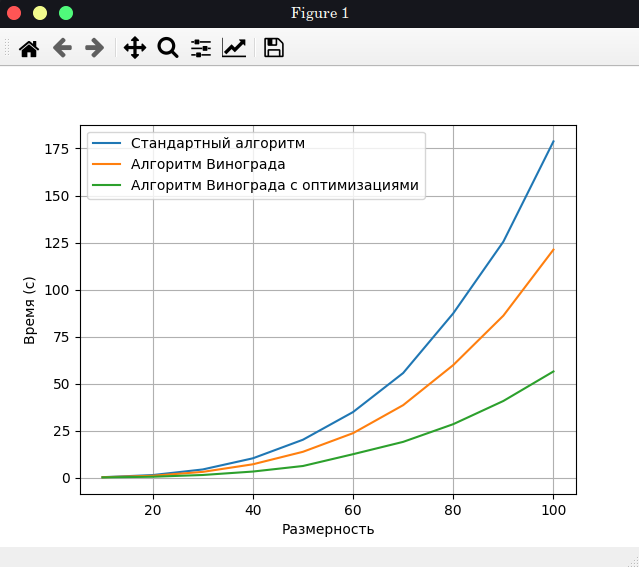
\includegraphics[width=0.8\textwidth]{time1.png}
		\caption{Временные характеристики на четных размерах матриц}
		\label{fg:ref3}}
\end{figure}

На рис. \ref{fg:ref4} показана работа алгоритмов с матрицами, размерностью [11, 21, 31,\dots,91].

\begin{figure}[ht!]
	\centering{
		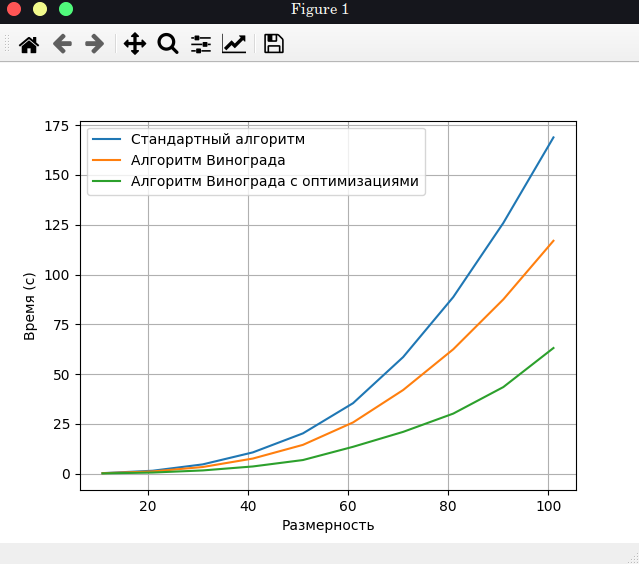
\includegraphics[width=0.8\textwidth]{time2.png}
		\caption{Временные характеристики на нечетных размерах матриц}
		\label{fg:ref4}}
\end{figure}

\section{Сравнительный анализ алгоритмов}

Введем модель вычислений трудоемкости алгоритма.
Пусть трудоемкость 1 у следующих базовых операций: +, -, *, /, \%, =, ==, !=, <, <=, >, >=, [].
%Трудоемкость цикла: fцикла = fиниц + fсравн + Nитер ∗ (fтела +
fинкрем + fсравн ).Трудоемкость условного перехода 1.

Стандартная реализация алгоритма не эффективна по времени, так как
обладает трудоемкостью 5qmn + 4n + 4mn + 5.
Оценка трудоемкости данного алгоритма составляет 5qmn. 
По памяти в стандартном алгоритме умножения матриц требуется m*n памяти под результат.

Теперь рассмотрим алгоритм Винограда умножения матриц. 
Реализация алгоритма Винограда обладает трудоемкостью формула \ref{eq:ref8}.
Оценка трудоемкости данного алгоритма составляет 3qmn.
В алгоритме Винограда умножения матриц требуется дополнительно m+n памяти под результат.

\begin{equation}
	3qmn + 7mn + 2m + 5q + 6n + 11 +
	\left[ 
	\begin{gathered} 
		0 $ л.с.$ \\ 
		5mn+4n+2 $ х.с.$ \\ 
	\end{gathered}
	\right.
	\label{eq:ref8}
\end{equation}

\section*{Вывод}

В данном разделе было произведено сравнение количества затраченного времени вышеизложенных алгоритмов.
Самым быстрым оказался модифицированный алгоритм Винограда.
При этом в алгоритме Винограда умножения матриц требуется дополнительно m+n памяти под результат.



\newpage
\chapter*{Заключение}
\addcontentsline{toc}{chapter}{Заключение}

В ходе работы были изучены алгоритмы умножения матриц. 
Реализованы 3 алгоритма, приведен программный код реализации алгоритмов по умножению матриц.
Была подсчитана трудоемкость каждого из алгоритмов. 
А также было проведено сравнение алгоритмов по времени и трудоемкости. Показано, что наименее трудоемкий и наименее затратный по времени при больших размерах матриц алгоритм Винограда оптимизированный.\\

Цель работы достигнута, решены поставленные задачи.
Получены практические навыки реализации алгоритмов Винограда и стандартного алгоритма, а также проведена 
исследовательская работа по оптимизации и вычислении трудоемкости алгоритмов.

\newpage
\renewcommand\bibname{Список литературы}
\addcontentsline{toc}{chapter}{Список литературы}
\makeatletter % список литературы
\def\@biblabel#1{#1. }
\makeatother
\begin{thebibliography}{2}
    \bibitem{analyse_info} Дж. Макконнел. Анализ алгоритмов. Активный обучающий подход. -- М.: Техносфера, 2017. -- 267с.
    \bibitem{anatyse_info}Основы программирования на языках Си и C++ для начинающих[Электронный ресурс]. Режим доступа: http://cppstudio.com/ (дата обращения 10.10.2021)
    \bibitem{analyse_info}LINUX.ORG.RU - Русскоязычная информация о ОС Linux[Электронный ресурс] Режим доступа://www.linux.org.ru/(дата обращения 25.10.2021)
    \bibitem{analyse_info} Погорелов Д. А. Таразанова А. М. Волкова Л. Л. Оптимизация классического алгоритма Винограда для перемножения матриц // Журнал №1 2019. Т. 49.
    \bibitem{}Корн Г., Корн Т. Алгебра матриц и матричное исчисление // Справочник по математике. — 4-е издание. — М.: Наука, 1978. — С. 392—394.
    
\end{thebibliography}

\end{document}
